\section{Metodologia experimental}\label{sec:metodologia}

\subsection{Caracterização da pesquisa}

Trata-se de uma pesquisa aplicada, de abordagem quantitativa, conduzida por
experimentos computacionais com um modelo de simulação estocástica. O
protocolo (hipóteses, sementes, métricas e testes) foi registrado no
repositório antes das rodadas definitivas (\texttt{docs/protocolo-experimental.md}).
As rodadas-piloto, usadas para depuração e para medir o custo computacional,
empregaram as sementes 1 e 3; as rodadas definitivas usam as sementes 1001 a
1030, e os resultados do piloto não entram em nenhuma análise.

\subsection{Modelos}

\paragraph{Geração de resíduos.}
Para o contêiner $i$, no passo $t$ do dia $d$ (dia da semana $w$, hora $h$), o
volume solto gerado, em litros, é
\begin{equation}
  q_{i,t} = \mu_i \, I \, W_{p_i}(w) \, Z_{i,d} \, H_{p_i}(h) \, E_{i,t} + e_{i,t},
  \label{eq:demanda}
\end{equation}
em que $\mu_i$ é a taxa média diária de longo prazo, $I$ é a intensidade do
cenário, $W_p$ e $H_p$ são os perfis semanal (média 1) e horário (soma 1) do
perfil $p_i \in \{$residencial, comercial, institucional$\}$, $Z_{i,d}$ e
$E_{i,t}$ são fatores Gama de média 1 que representam a variação entre dias
(CV 0,25) e a chegada irregular dos descartes ao longo do dia (CV 1,0), e
$e_{i,t}$ representa descartes volumosos esporádicos (processo de Poisson, em
média um a cada 30 dias por contêiner, com 15\% a 45\% do volume do
contêiner). A heterogeneidade entre contêineres é dada por
$\mu_i = \bar\mu_{p_i}\,\eta_i$, com $\eta_i$ lognormal de média 1 e CV 0,35.
A distribuição Gama foi escolhida por ser não negativa e permitir controlar a
média e o coeficiente de variação de forma independente; a lognormal, por
produzir a assimetria à direita esperada entre pontos de coleta.

\paragraph{Estado do contêiner e transbordamento.}
A ocupação verdadeira $f_i \in [0,1]$ evolui como $f_i \leftarrow f_i +
q_{i,t}/V$. Se o resultado excede 1, o excedente $(f_i-1)V$ é contabilizado
como volume transbordado e $f_i$ é limitado a 1. O modelo, portanto, não
supõe que o resíduo excedente seja recolhido depois; ele representa uma falha
de serviço. Uma coleta zera $f_i$.

\paragraph{Sensor ultrassônico.}
Com contêiner prismático de seção constante, a fração de volume é igual à
fração de altura (Figura~\ref{fig:conteiner}). Com $D_0$ a distância do sensor
ao fundo, $\mathit{off}$ a zona morta de montagem e $H = D_0 - \mathit{off}$,
a distância verdadeira até a superfície é $d = D_0 - f H$, e a ocupação
calculada pelo firmware e pela plataforma é
\begin{equation}
  \hat o(d) = 100 \cdot \min\!\left\{1, \max\!\left\{0, \frac{H - (d - \mathit{off})}{H}\right\}\right\},
  \label{eq:ocupacao}
\end{equation}
considerada inválida se $d$ estiver fora de $[2, 400]$~cm ou além do fundo
($d > D_0 + 15$~cm). A medição simulada é
\begin{equation}
  d^{\mathrm{med}} = d + \sigma_r\,\varepsilon_1 - \sigma_s\,|\varepsilon_2|,\qquad
  \varepsilon_1,\varepsilon_2 \sim \mathcal N(0,1),
  \label{eq:sensor}
\end{equation}
em que o termo semi-normal negativo representa o retorno do primeiro eco pelo
ponto mais alto de uma superfície irregular e produz um viés de
superestimação da ocupação de $\sigma_s\sqrt{2/\pi}$. Com probabilidade de 1\%
a leitura é perdida (sem eco) e com 0,5\% é espúria, entre 3 e 20~cm,
simulando uma obstrução momentânea. A
Figura~\ref{fig:sensor}(b) mostra 1.500 leituras simuladas nos níveis base e
de ruído seis vezes maior. A formulação não se aplica a geometrias não
prismáticas sem uma curva altura--volume específica.

\begin{figure}[ht]
  \centering
  % Modelo geométrico do contêiner instrumentado
\begin{tikzpicture}[font=\sffamily\scriptsize, >={Stealth[length=1.6mm]}]
\def\W{3.2}\def\Hb{4.4}\def\off{0.4}\def\fl{1.9}
\fill[brown!35] (0,0) -- (\W,0) -- (\W,\fl) .. controls (2.2,\fl+0.35) and (1.2,\fl-0.25) .. (0,\fl+0.1) -- cycle;
\draw[thick] (0,\Hb) -- (0,0) -- (\W,0) -- (\W,\Hb);
\draw[thick] (-0.15,\Hb) -- (\W+0.15,\Hb);
\node[draw, fill=blue!15, minimum width=10mm, minimum height=3mm, inner sep=0] (s) at (\W/2,\Hb-0.15) {};
\node[above=1mm of s] {HC-SR04};
\fill[blue!8, opacity=.6] (\W/2-0.08,\Hb-0.3) -- (\W/2-0.08-0.55,1.95) -- (\W/2+0.08+0.55,2.05) -- (\W/2+0.08,\Hb-0.3) -- cycle;
\node[blue!60!black] at (\W/2+0.95,3.0) {cone $\approx 15^\circ$};
\draw[dashed, gray] (0,\Hb-\off) -- (\W,\Hb-\off);
\draw[<->] (\W+0.5,0) -- node[right] {$D_0$} (\W+0.5,\Hb-0.3);
\draw[<->] (\W+1.2,\Hb-0.3) -- node[right] {$\mathit{off}$} (\W+1.2,\Hb-\off);
\draw[<->] (\W+1.2,0) -- node[right] {$H = D_0-\mathit{off}$} (\W+1.2,\Hb-\off);
\draw[<->, red!70!black] (\W/2+0.15,\Hb-0.3) -- node[right] {$d$} (\W/2+0.15,2.08);
\draw[<->] (-0.4,0) -- node[left, align=right] {altura\\ocupada\\$h$} (-0.4,\fl);
\node[align=center] at (\W/2,0.7) {resíduos\\(superfície irregular)};
\end{tikzpicture}

  \caption{Geometria adotada para o contêiner instrumentado.}
  \label{fig:conteiner}
\end{figure}

\begin{figure}[ht]
  \centering
  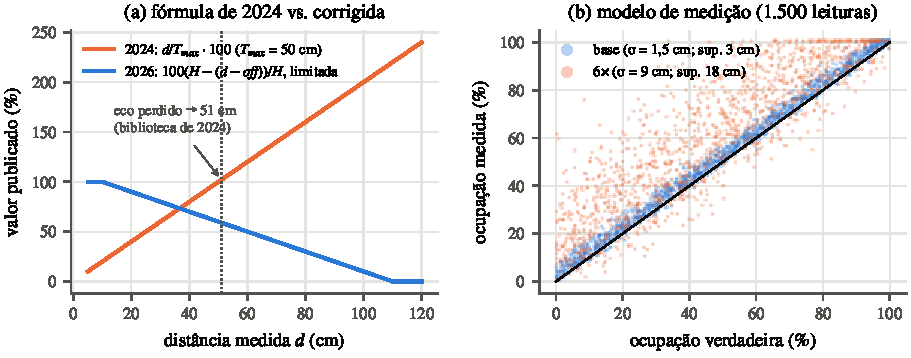
\includegraphics[width=\textwidth]{figures/fig_sensor.pdf}
  \caption{(a) Valor publicado em função da distância medida: a fórmula de 2024
  cresce quando o contêiner esvazia e ultrapassa 100\%; a fórmula corrigida
  é limitada a $[0,100]$. (b) Ocupação medida $\times$ verdadeira pelo modelo
  de sensor (Equação~\ref{eq:sensor}), nos níveis de ruído base e 6$\times$.}
  \label{fig:sensor}
\end{figure}

\paragraph{Disponibilidade e canal.}
Cada dispositivo alterna entre operacional e indisponível segundo uma cadeia
de Markov de dois estados, com tempo médio entre falhas de 60 dias e tempo
médio de reparo de 12~h. Opcionalmente, uma fração dos dispositivos falha
definitivamente em instante uniforme no horizonte, ou passa a repetir a mesma
leitura (sensor ``congelado''). Cada mensagem é perdida com probabilidade
$p_{\mathrm{perda}}$, duplicada com probabilidade 0,2\% e atrasada segundo uma
lognormal de mediana 0,5~s, com 0,2\% de atrasos longos (1 a 6~h). Interrupções
regionais tornam inacessíveis os dispositivos mais próximos de um centro
sorteado durante um intervalo; o firmware não armazena leituras para reenvio,
de modo que as mensagens desse período são perdidas.

\paragraph{Planejamento e execução.}
As políticas e a formulação do CVRP com prêmios foram apresentadas na
Seção~\ref{sec:politicas} (Equação~\ref{eq:objetivo}).

\subsection{Cenário, dados e parâmetros}\label{sec:parametros}

O cenário usa a malha viária dirigível do município de Aracaju, extraída do
OpenStreetMap \cite{haklay2008openstreetmap} a partir do extrato da região
Nordeste distribuído pela Geofabrik \cite{geofabrik2026nordeste}, com
integridade conferida por MD5. O limite municipal é a relação administrativa
do próprio OSM. Mantiveram-se as vias de uso automotivo, os sentidos de
circulação e a maior componente fortemente conexa: \num{45011} nós,
\num{86410} arcos dirigidos e \num{3058,7}~km de arcos. Os contêineres são
posicionados em interseções sorteadas (uniformemente, ou em agrupamentos no
experimento E4), o que faz a densidade de contêineres acompanhar a densidade
de ruas. O depósito é o nó mais próximo de um ponto hipotético no oeste da
área urbana (Figura~\ref{fig:cenario}). As distâncias são caminhos mínimos na
malha dirigida, calculados pelo algoritmo de Dijkstra (SciPy
\cite{virtanen2020scipy}).

\begin{figure}[ht]
  \centering
  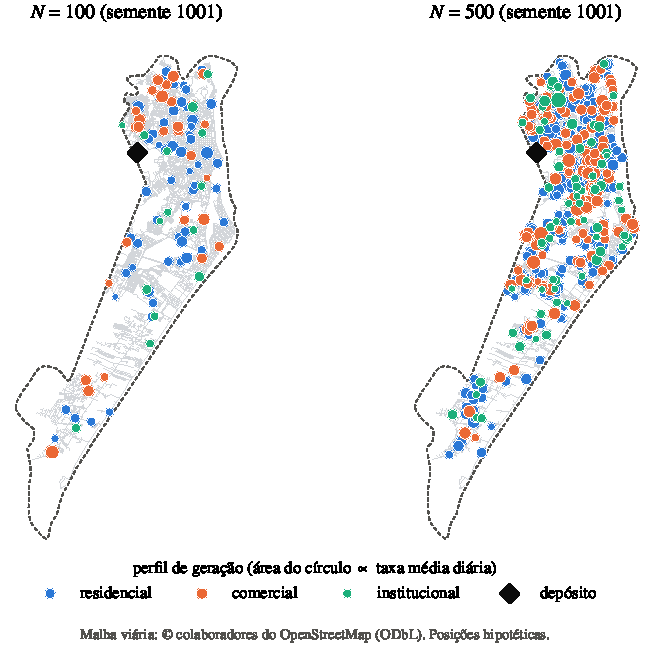
\includegraphics[width=0.92\textwidth]{figures/fig_cenario.pdf}
  \caption{Contêineres simulados sobre a malha viária de Aracaju para 100 e 500
  contêineres (semente 1001). As posições e o depósito são hipotéticos e não
  correspondem a equipamentos existentes.}
  \label{fig:cenario}
\end{figure}

A Tabela~\ref{tab:parametros} separa os parâmetros segundo sua natureza: dado
público observado (P), dado geográfico real (G), valor da literatura (L),
hipótese de cenário (H) e dado sintético (S). Os parâmetros de demanda são
hipóteses ancoradas em dados oficiais: com geração domiciliar de 0,88
kg/hab$\cdot$dia no Nordeste \cite[p.~26]{brasil2025sinisa} e densidade
aparente de 230~kg/m³ \cite{monteiro2001manual}, cada habitante gera cerca de
3,8~L/dia de resíduo solto, e um contêiner com taxa média de 300~L/dia
atenderia cerca de 78 pessoas. Não há dado municipal verificado de geração por
contêiner em Aracaju, e os perfis semanais e horários não foram calibrados com
medições; por isso, as conclusões são apresentadas como condicionais a esses
parâmetros, e os mais influentes são variados em E3 e E4.

\begin{table}[ht]
\centering
\caption{Parâmetros principais e sua natureza (P: dado público; G: geográfico real; L: literatura; H: hipótese; S: sintético). Lista completa em \texttt{docs/parametros.md}.}
\label{tab:parametros}
\scriptsize
\begin{tabularx}{\textwidth}{@{}>{\raggedright\arraybackslash}p{3.3cm}>{\raggedright\arraybackslash}p{3.0cm}c>{\raggedright\arraybackslash}X@{}}
\toprule
Parâmetro & Valor-base & Nat. & Fonte ou justificativa \\
\midrule
Malha viária & Aracaju, OSM, 45.011 nós & G & \cite{geofabrik2026nordeste} \\
Posição de contêineres e depósito & interseções sorteadas & S & hipotético \\
Geração domiciliar per capita & 0,88 kg/hab$\cdot$dia & P & \cite{brasil2025sinisa} (contexto) \\
Densidade aparente (solto) & 230 kg/m³ & L & \cite{monteiro2001manual} \\
Volume do contêiner & 1.100 L & L & \cite{monteiro2001manual} \\
Geometria & prismática; $D_0$ = 110 cm; $\mathit{off}$ = 10 cm & H & simplificação \\
Taxa média por perfil & 300 / 380 / 260 L/dia & H & $\approx$ 78 hab./contêiner \\
Mistura de perfis & 60\% / 25\% / 15\% & H & --- \\
Variabilidade & lognormal CV 0,35; Gama CV 0,25 e 1,0 & H & --- \\
Faixa do HC-SR04 & 2--400 cm & L & \cite{elecfreakssdhcsr04} \\
Ruído; irregularidade da superfície & $\sigma_r$ = 1,5 cm; $\sigma_s$ = 3 cm & H & variado em E3 \\
Leituras perdidas / espúrias & 1\% / 0,5\% & H & variado em E3 \\
MTBF / MTTR do dispositivo & 60 dias / 12 h & H & --- \\
Período de medição & 60 min & H & variado em E3 \\
Perda de mensagens & 1\% & H & variado em E3 \\
Capacidade do caminhão & 26.000 L soltos ($\approx$ 6 t) & L+H & 15 m³ \cite{monteiro2001manual} $\times$ 400 kg/m³ \cite{epa2016volume} $\div$ 230 kg/m³ \\
Tempo de atendimento & 60 s & L+H & 41,95 s medidos \cite{carlos2019influence} + posicionamento \\
Descarga & 15 min & L & \cite{monteiro2001manual} \\
Velocidade média & 20 km/h & H & variada em E4 \\
Jornada & 8 h (07h--15h) & H & --- \\
Frota & $\lceil \sum_i \mu_i / (0{,}7\,Q)\rceil$ & H & mesma para todas as políticas \\
Limiares & $\theta_{hi}$ = 0,75; $\theta_{lo}$ = 0,50; $\theta_{crit}$ = 0,95 & H & 70--75\% em \cite{akhtar2017backtracking}; varridos em E2 \\
\bottomrule
\end{tabularx}
\end{table}

A frota é dimensionada pela demanda média total, com utilização-alvo de 70\%,
e é a mesma para todas as políticas de um cenário. Com essa regra, os cenários
de 20, 100 e 500 contêineres usam \VehNVinteA{}, \VehNCemA{} e
\VehNQuinhentosA{} veículos, respectivamente. Como a área do município é fixa,
o número de contêineres altera também a densidade espacial: em $N = 20$, os
pontos estão distantes entre si, situação que favorece pouco a seleção
dinâmica.

\subsection{Experimentos}

A Figura~\ref{fig:protocolo} resume os seis experimentos. Cada execução simula
7 dias de aquecimento, descartados, seguidos de 28 dias avaliados (quatro
semanas completas, de modo que todos os dias da semana têm o mesmo peso). O
aquecimento elimina a influência do enchimento inicial (uniforme entre 0 e
50\%) e do estado inicial da plataforma, que começa sem histórico.

\begin{figure}[ht]
  \centering
  \resizebox{\textwidth}{!}{% Protocolo experimental
\begin{tikzpicture}[font=\sffamily\scriptsize, node distance=3mm and 4mm,
  e/.style={draw, rounded corners=2pt, text width=34mm, align=left, inner sep=3pt, fill=#1, minimum height=15mm},
  arr/.style={-{Stealth[length=1.8mm]}, thick}]
\node[draw, rounded corners=2pt, fill=gray!10, text width=118mm, align=center] (base) {Cenário-base: malha de Aracaju (OSM), contêineres hipotéticos de 1.100 L, 7 dias de aquecimento + 28 dias avaliados; sementes 1001--1030; números aleatórios comuns; métricas primárias: km/dia e transbordamento (\% do volume gerado)};
\node[e=red!6, below left=4mm and -38mm of base] (e1) {\textbf{E1} comparação principal\\$N\in\{20,100,500\}$\\A, B, B-OR, C, D\\30 sementes (450 execuções)};
\node[e=red!6, right=of e1] (e2) {\textbf{E2} fronteiras km $\times$ serviço\\5--7 níveis de limiar\\A, B-OR, C, D; 20 sementes (440)};
\node[e=red!6, right=of e2] (e3) {\textbf{E3} robustez da telemetria\\perda, interrupções, ruído, falhas, amostragem, \emph{fallback}\\30 sementes (1.860)};
\node[e=red!6, below=of e1] (e4) {\textbf{E4} sensibilidade\\demanda, variabilidade, mudança de regime, frota, layout, velocidade\\30 sementes (1.200)};
\node[e=red!6, right=of e4] (e5) {\textbf{E5} solver\\descida gulosa $\times$ GLS (5 s)\\$N=500$; 10 sementes (60)};
\node[e=blue!8, right=of e5] (e6) {\textbf{E6} MQTT real\\entrega e latência, equivalência, reinício do broker, LWT, mensagens inválidas};
\node[draw, rounded corners=2pt, fill=green!8, text width=118mm, align=center, below=4mm of e5] (st) {Análise pareada por semente: IC 95\% \emph{bootstrap} da diferença média; Wilcoxon bilateral; correção de Holm por família; correlação bisserial de postos; balanço de volume verificado em todas as execuções};
\draw[arr] (base.south) -- ++(0,-2mm);
\end{tikzpicture}
}
  \caption{Protocolo experimental.}
  \label{fig:protocolo}
\end{figure}

\begin{description}
  \item[E1 -- comparação principal.] Políticas A, B, B-OR, C e D com 20, 100 e
  500 contêineres; 30 sementes por combinação (\NExecEUm{} execuções).
  \item[E2 -- fronteira distância $\times$ serviço.] Com 100 contêineres, cada
  política é executada em vários níveis de seu parâmetro de agressividade:
  ocupação-alvo $\gamma \in \{0{,}4; \dots; 1{,}0\}$ para A e limiar
  $\theta_{hi} \in \{0{,}5; \dots; 0{,}9\}$ para B-OR, C e D (com $\theta_{lo}
  = \theta_{hi} - 0{,}25$ e $\theta_{crit} = \theta_{hi} + 0{,}2$);
  20 sementes (\NExecEDois{} execuções). O objetivo é comparar políticas no
  mesmo nível de serviço, e não apenas em seus parâmetros padrão.
  \item[E3 -- robustez da telemetria.] Com 100 contêineres, fatores variados um
  de cada vez: perda de mensagens (5\%, 20\%, 50\%); interrupções regionais de
  48~h atingindo 50\% dos dispositivos, em média uma vez por semana; medição
  ideal (sem ruído, sem viés de superfície e sem leituras inválidas ou
  espúrias) e ruído 3$\times$ e 6$\times$ ($\sigma_r$ e $\sigma_s$ multiplicados); falha permanente de 10\% e 30\% dos dispositivos;
  10\% de sensores congelados; período de medição de 15~min, 6~h e 24~h; e
  desativação do \emph{fallback} nas condições de falha de 30\% e de
  interrupção; 30 sementes (\NExecETres{} execuções).
  \item[E4 -- sensibilidade operacional.] Com 100 contêineres: intensidade de
  demanda 0,7 e 1,3 (com frota redimensionada); alta variabilidade (CV diário
  0,5, CV intradiário 2,0, descartes volumosos a cada 10 dias); mudança de
  regime (+60\% de geração em 30\% dos contêineres a partir do dia 14) e surto
  geral (+30\% em todos), ambos não antecipados pelo calendário de A nem pelo
  dimensionamento da frota; frota reduzida a um veículo; layout
  agrupado; e velocidades de 15 e 30~km/h; 30 sementes (\NExecEQuatro{} execuções).
  \item[E5 -- resolvedor.] Descida gulosa $\times$ busca local guiada com
  limite de 5~s por dia, para A, C e D com 500 contêineres; 10 sementes
  (\NExecECinco{} execuções).
  \item[E6 -- integração MQTT.] Broker Mosquitto real: entrega e latência com
  100 dispositivos virtuais em QoS~0 e QoS~1 (três repetições); equivalência
  entre o modo \emph{live} e o modo em lote com canal ideal; reinício do broker
  durante a publicação; queda abrupta de 10 dispositivos (LWT); e 50 mensagens
  malformadas.
\end{description}

\subsection{Métricas}

As métricas primárias são a \textbf{distância percorrida} (km/dia, incluindo
desvios de descarga e retorno ao depósito) e o \textbf{transbordamento}, isto
é, o volume que não coube nos contêineres, em percentual do volume gerado no
período avaliado. As duas são analisadas em conjunto, porque uma política que
deixa de atender contêineres percorre menos e transborda mais.

As métricas secundárias são: visitas por dia; km por m³ coletado; número de
episódios em que um contêiner atinge a capacidade; horas de contêiner cheio
por contêiner e dia; ocupação verdadeira média no momento da coleta;
percentual de coletas com ocupação abaixo de 50\%, aqui chamadas de
\emph{coletas prematuras}; tempo médio entre um contêiner cruzar 80\% e ser
coletado; utilização da capacidade dos veículos (volume coletado dividido
pelo número de viagens vezes $Q$); viagens extras de descarga; visitas
planejadas não realizadas; contêineres obrigatórios descartados pelo
planejador; tempo de execução do resolvedor; disponibilidade de telemetria
(leituras válidas entregues sobre leituras programadas); e o erro absoluto
médio da previsão de ocupação com 24~h de antecedência, comparado ao da
persistência (supor que a ocupação não muda), calculado apenas para
contêineres sem coleta no intervalo. Estimativas de combustível e emissões não
são usadas como métrica: a única fonte verificada para o consumo de
caminhões compactadores foi lida apenas no resumo e refere-se a outro país
\cite{nguyen2010fuel}.

\subsection{Análise estatística}

Para cada condição, são calculados média, desvio-padrão, mediana, quartis e
intervalo de confiança de 95\% da média por \emph{bootstrap} percentil, com
\num{10000} reamostragens e semente fixa
\cite{efron1979bootstrap,efron1993introduction}. As comparações pré-definidas
(B, B-OR, C e D contra A; D contra C; C contra B-OR; B-OR contra B) são
pareadas por semente. Para cada uma, reporta-se a diferença média com IC de
95\% por \emph{bootstrap}, a diferença relativa, o teste de postos sinalizados
de Wilcoxon bilateral \cite{wilcoxon1945individual} e a correlação bisserial
de postos pareada $r_{rb}$ \cite{kerby2014simple}, em que $r_{rb} = -1$
significa que a política alternativa teve valor menor que a de referência em
todas as sementes. Os valores $p$ são ajustados pelo procedimento de Holm
\cite{holm1979simple} dentro de cada família, definida como a combinação de
experimento e métrica. Testes de normalidade não foram usados para escolher o
teste: o Wilcoxon foi definido de antemão por não exigir normalidade das
diferenças. No E2, o desempenho no mesmo nível de serviço é obtido por
interpolação linear, para cada semente e política, da distância necessária
para transbordamento de 1\% e de 2\% do volume; sementes em que o nível não é
alcançado dentro da faixa varrida são excluídas da comparação, e seu número é
informado.

\subsection{Verificação, reprodutibilidade e ameaças à validade}

\paragraph{Verificação.}
Além dos testes automatizados, cada execução verifica o balanço de volume. Em
todas as \NExecTotal{} execuções, o maior resíduo absoluto foi de
\BalancoMaxResidual{}~L, compatível com erro de arredondamento em ponto
flutuante. O roteirizador foi comparado à enumeração exata em instâncias
pequenas, e os comprimentos das rotas reconstruídas pela malha coincidiram com
os usados pelo otimizador.

\paragraph{Reprodutibilidade.}
Cada execução é determinada pela configuração completa e pela semente,
gravadas junto com as métricas. Os resultados brutos, o manifesto (versão do
código, dependências, plataforma) e os scripts de análise estão no
repositório. A descida gulosa do OR-Tools foi escolhida por ser determinística.
Uma amostra das execuções foi repetida com a versão final do código, como
descrito na Seção~\ref{sec:resultados}.

\paragraph{Desvio do protocolo.}
Depois do início das rodadas definitivas, o código foi submetido a uma revisão
independente, feita por um revisor que não participou da implementação. Ela
encontrou quatro problemas, corrigidos antes da conclusão das rodadas e
registrados em \texttt{docs/desvios-protocolo.md}. (i)~A política A usava a
taxa média de geração sem os descartes volumosos (cerca de 3,5\% do volume no
cenário-base), contrariando a premissa de histórico perfeito e desfavorecendo
A; todas as execuções de A foram refeitas, e as anteriores foram arquivadas sem
uso. (ii)~A grade de limiares do E2 não levava todas as políticas a atravessar
1\% e 2\% de transbordamento, o que restringia a comparação no mesmo nível de
serviço a um subconjunto não aleatório de sementes; foram acrescentados os
níveis 0,3 e 0,4 (B-OR e C) e 1,0 (D). (iii)~A condição ``frota reduzida'' do
E4 resultava na mesma frota da base e foi redefinida como um único veículo.
(iv)~No E5, o limite de tempo de 5~s truncaria também a descida gulosa, que
passou a usar a mesma salvaguarda de 30~s do E1. A revisão confirmou, por
outro lado, a ausência de vazamento do estado verdadeiro para as políticas
B--D, a validade dos números aleatórios comuns entre políticas e a correção
das unidades do modelo de roteirização e dos procedimentos estatísticos.

\paragraph{Ameaças à validade.}
\emph{Interna}: os perfis de geração são hipóteses; o passo de 15~min
discretiza os instantes de coleta; o resolvedor é heurístico, e diferenças de
qualidade de rota podem se confundir com diferenças de política (mitigado pela
variante B-OR e pelo E5); B e C estimam a carga dos veículos pelo nível
observado no planejamento, e não pelo nível esperado na visita, o que lhes
impõe mais desvios de descarga; a taxa inicial da ingestão é a mediana
verdadeira das taxas, efeito restrito ao aquecimento descartado; e, na condição
de amostragem a cada 15~min, os sorteios de ruído e falhas diferem dos da base,
o que enfraquece o pareamento dessa condição. \emph{De construto}: o transbordamento é modelado
como volume recusado, sem efeito sobre o tempo de atendimento; o limiar de
50\% para ``coleta prematura'' é arbitrário, e por isso a distribuição completa
da ocupação na coleta também é apresentada; a espera considera apenas
episódios encerrados por coleta; e a disponibilidade de telemetria inclui
leituras válidas que chegam atrasadas e são descartadas pela ingestão. \emph{Externa}: os contêineres e o
depósito são hipotéticos; a velocidade é constante e não há trânsito; cada
veículo tem uma viagem planejada por turno, com desvios de descarga apenas
quando necessário; não há restrições de janela de horário; a política A usa
taxas médias verdadeiras, o que a favorece. \emph{De conclusão}: as
comparações são pareadas e ajustadas para multiplicidade, mas os fatores de E3
e E4 foram variados um de cada vez, e interações não foram estimadas.
